\section{Data Analysis}
Data analysis is a critical step in understanding the underlying quality, patterns, and characteristic of the dataset.

\subsection{Data Quality Check}
Ensuring high data quality is a critical first step before any analysis.
In this stage, the following checks are performed:
\begin{itemize}
    \item \textbf{Missing Values:} Confirm that there are no missing entries, or if there are, decide on an appropriate imputation method.
    \item \textbf{Outliers:} Identify any extreme values using statistical methods (this project used IQR), or if there are any, determine if they need to be removed or capped.
    \item \textbf{Duplicates:} Check for duplicate records to prevent bias in analysis.
    \item \textbf{Consistency and Integrity:} Ensure data types, ranges, and formats are consistent across the dataset.
\end{itemize}

\subsection{Exploratory Data Analysis}
Exploratory Data Analysis (EDA) involves summarizing the main characteristics of the dataset using visual and quantitative methods.
This project includes the following EDA techniques:
\begin{itemize}
    \item \textbf{Summary Statistics:} Compute mean, median, variance, and other descriptive measures to understand data distribution.
    \item \textbf{Line Chart for Long-Term Trends:} Plot the USDEUR exchange rate over time to reveal long-term trends and identify potential anomalies. (See Figure~\ref{fig:line_chart}.)
\end{itemize}

\begin{figure}[H]
\centering
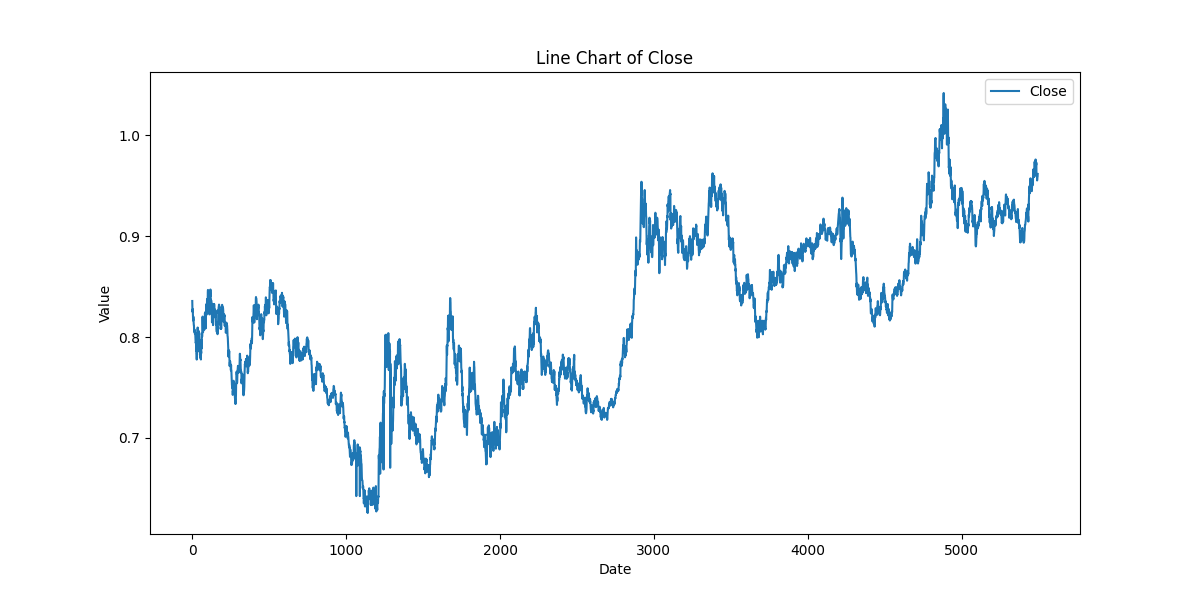
\includegraphics[width=\textwidth]{figures/line_chart}
\caption{Line Chart of the USDEUR Exchange Rate (The Primary Dataset)}
\label{fig:line_chart}
\end{figure}

\textcolor{red}{QUESTION: Caption like this, should I write them more carefully?}

\subsection{Stationarity Testing}
Stationarity testing is an important process in time series analysis.
A stationary time series has constant statistical properties (mean, variance, autocorrelation) over time.
Testing for stationarity helps make decision, such as if differencing or detrending are necessary.

\subsubsection{Augmented Dickey-Fuller Test}
The Augmented Dickey-Fuller (ADF) test is a widely-used statistical test to assess the presence of a unit root in a time series sample.
It operates under the following principles:
\begin{itemize}
    \item \textbf{Null Hypothesis (H\(_0\)):} The time series has a unit root, which means it is non-stationary.
    \item \textbf{Alternative Hypothesis (H\(_1\)):} The time series is stationary.
    \item \textbf{Mechanism:} The ADF test augments the standard Dickey-Fuller test by including lagged difference terms to account for higher order autoregressive processes.
    If the test statistic is significantly lower than the critical values, we reject the null hypothesis and conclude that the series is stationary.
    Otherwise, we fail to reject the null hypothesis.
\end{itemize}

\subsubsection{Kwiatkowski-Phillips-Schmidt-Shin Test}
The Kwiatkowski-Phillips-Schmidt-Shin(KPSS) test complements the ADF test by taking the opposite approach:
\begin{itemize}
    \item \textbf{Null Hypothesis (H\(_0\)):} The time series is stationary around a deterministic trend (or level stationary).
    \item \textbf{Alternative Hypothesis (H\(_1\)):} The time series is non-stationary.
    \item \textbf{Mechanism:} The KPSS test evaluates the null hypothesis by estimating the variance of a random walk component in the series.
    If the test statistic exceeds the critical value, we reject the null hypothesis and conclude that the series is non-stationary.
    Otherwise, we fail to reject the null hypothesis.
    This test is particularly useful because it provides a different perspective on stationarity compared to the ADF test.
\end{itemize}
